\subsection{データの抽象化入門}
プロシージャーを作ることによって, 複合の操作だけでなく,
抽象化として見ることができる.

複合のデータについても同じことができ, それをデータの抽象化という.
プログラムにおいて, 抽象的にデータを扱うというのは,
可能な限りデータはどう表現されているか関係なく扱うことである.
それに対して, 具体的なデータはプログラムと関係なく定義されているものである.

具体的なデータと抽象的なデータの間に変換するために, セレクターとコンストラクタを用いる.
%
\subsubsection{有理数での算術}
有理数を使って四則演算を実装したいとする. 分数を表す方法がある前提で考えて,
分子と分母から分数を返す\lstinline{make-rat}, 分数から分子を返す\lstinline{numer},
分数から分母を返す\lstinline{denom}という3つのプロシージャが存在するとする.

分数の四則演算は

\begin{align*}
  &\frac{n_1}{d_1} + \frac{n_2}{d_2}  = \frac{n_1d_2 + n_2d_1}{d_1d_2}
  & \frac{n_1}{d_1}\cdot \frac{n_2}{d_2} = \frac{n_1n_2}{d_1d_2}\\
  &\frac{n_1}{d_1} - \frac{n_2}{d_2} = \frac{n_1d_2 - n_2d_1}{d_1d_2}
  & \frac{n_1/d_2}{n_2/d_2} = \frac{n_1d_2}{d_1n_2}\\
  &\frac{n_1}{d_1} = \frac{n_2}{d_2} \Leftrightarrow n_1d_2 = n_2d_1
\end{align*}
\noindent
のように定義できるので, 以上の3つのプロシージャがあれば, 問題なくそれぞれの
演算を問題なく実装できる. 例えば, 足し算は以下のように実装できる.

\begin{lstlisting}[basicstyle=\footnotesize,title=分数の足し算]
(define (add-rat x y)
  (make-rat (+ (* (numer x) (denom y))
               (* (numer y) (denom x)))
            (* (denom x) (denom y))))
\end{lstlisting}
\vspace{5mm}

Lispにはペアというデータ構造が存在しており, 2つのデータを1つの構造として表現できる.
\lstinline{cons}で2つの要素から1つのペアを作ることができ, \lstinline{car}で
1つ目の要素を取り出し, \lstinline{cdr}で2つ目の要素を取り出す.
ペアを用いると, 分数を自然に表現することができる.

\begin{lstlisting}[basicstyle=\footnotesize,title=分数の表現]
(define (make-rat n d) (cons n d))
(define (numer x) (car x))
(define (denom x) (cdr x))
\end{lstlisting}

%
\subsubsection{抽象化の壁}
データを扱う時に複数の抽象化のレイヤについて考えられる.
分数の例で考えると, 以下の図のようなレイヤが考えられる.

\begin{figure}[h]
  \centering
  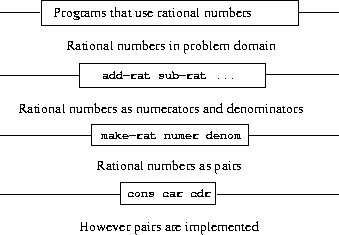
\includegraphics[width=12cm,height=5cm]{imgs/abstraction-barrier.png}
\end{figure}

ここで抽象化のレベルが4つで分かれている. 最も上のレイヤは分数を扱うプログラムが使うもので,
実際分数はどう表現されているかも, どう四則演算が定義されているのかが分からなくても四則演算が
できるレベルである. その下のレイヤでは, 実際四則演算の実装である. そこで分数のセレクタと
コンストラクタを用いるが, その実装に依存しない. その下のレイヤはセレクタとコンストラクタの実装で,
ペアを用いるが今回もその実装に依存しない. 最も下のレイヤはペアの実装である.

そのレイヤ分けの主な利点はプログラムの保守性と柔軟性の向上である.
下のレイヤの実装に依存しないので, データをどう表現するかが変わらない限り,
実装が変わっても影響が受けない.

%
\subsubsection{データとは}
以上で,セレクタとコンストラクタを用いて具体的なデータを抽象的なデータに
変換できることがわかったが, 抽象的なデータについて定義を固める必要がある.

\noindent
先ほどまでの例において、有理数はコンストラクタ(\lstinline{make-rat})と
セレクタ(\lstinline{numer}、\lstinline{denom})を用いて扱うことができた。
しかし、任意の三つの手続きの組が、有理数の実装に使えるわけではなく、
${}^{\forall} ($\lstinline{n}$, $\lstinline{d}$)
\in (\mathbb{N}\times \mathbb{N}\backslash \{0\})$
に対して, 次の関係が満たされる必要がある.
\[
  \text{\lstinline{x = (make-rat n d)}} \Leftrightarrow
  \frac{\text{\lstinline{numer x}}}{\text{\lstinline{denom x}}}
  = \frac{\text{\lstinline{n}}}{\text{\lstinline{d}}}
\]

従って、データとはコンストラクタとセレクタの集合と、それらのプロシージャ
がデータを正しく表現するための条件によって定義される。

この定義は、有理数のようなハイレベルなデータだけではなく、ローレベルな
データについても有効である。

例えば、有理数の実装に用いた「ペア」というデータ構造について考えてみる。
我々は今まで言語実装のコンストラクタ(\lstinline{cons})と
セレクタ(\lstinline{car}、\lstinline{cdr})を用いて扱ってきた。
重要なのはそれらのプロシージャがどう実装されているかではなく、
以下のような条件を満たしているかどうかである。

\[
  \text{\lstinline{z = (cons x y)}} \Rightarrow
  \text{\lstinline{(car z) = x}} \ \text{\lstinline{and}} \ \text{\lstinline{(cdr z) = y}}
\]

つまり、これらの条件を満たせば、言語レベルのデータ構造を用いずとも、
プロシージャのみを用いて実装することが可能である。

以下に、プロシージャを用いた有理数のためのコンストラクタ及びセレクタの定義を示す。

\begin{lstlisting}[basicstyle=\footnotesize,title=プロシージャによるペアの実装]
(define (cons x y)
  (define (dispatch m)
    (cond ((= m 0) x)
          ((= m 1) y)
          (else (error ``Argument not 0 or 1 -- CONS'' m))))

(define (car z) (z 0))

(define (cdr z) (z 1))
\end{lstlisting}
\vspace{5mm}

これにより、プロシージャを用いて、先に述べた条件を満たすコンストラクタ
とセレクタを定義することができることをわかった(ただし、ほとんどの言語では
効率の観点からペアを直接実装している)。この例は、プロシージャを第一級として
扱える能力が、自動的に、合成データをも表現できる能力となることも示している。
このプログラミング手法はしばしばメッセージパッシングスタイルと呼ばれ、
モデリングとシミュレーションについて論ずる第3章において基礎的なツール
として使われることになる。

